\documentclass[a4paper,11pt]{article}

\usepackage[english, portuguese]{babel}
%\usepackage[portuguese]{babel}
\usepackage[T1]{fontenc}
\usepackage{amsmath, amssymb}
\usepackage{graphicx}
\usepackage[utf8]{inputenc}
\usepackage{color}
\usepackage{listings}
\usepackage{float}

\lstset{
    backgroundcolor=\color[rgb]{0.86,0.88,0.93},
    language=R, keywordstyle=\color[rgb]{0,0,1},
    basicstyle=\footnotesize \ttfamily,breaklines=true,
    escapeinside={\%*}{*)}
}

\begin{document}

%%%%%%%%%% Headings page %%%%%%%%%%%
\begin{figure}[!h] 
\includegraphics [scale=0.3] {Course-name} \end{figure}
%\pagestyle{empty}
{\Large \noindent \bf Homework III} 
\vskip0.8cm

%%%%%%%%%% Guidelines %%%%%%%%%%%
{\Large \noindent \bf Guidelines} \\

\noindent You must solve each exercise using hand calculations and compare your results on Matlab/Octave. The report for the homework must be sent in a {\bf single pdf document} by {\bf July 10, 2017}. Note that {\bf late submissions will not be considered}. \\

\noindent Your report must include:
\begin{itemize}
\item The relevant steps, the results and your comments on each exercise.
\item The Matlab/Octave code developed for solving each exercise. This can be included as part of the single exercise or in a separate section of the report (for instance, as an appendix).
\item The graphs required in each exercise. 
\end{itemize}

\vskip0.8cm

%%%%%%%%%% Ex 1 %%%%%%%%%%%
{\Large \noindent \bf Exercise 1} \hfill					25 Points\\

\noindent  Consider the negative feedback system shown in Figure \ref{fig:ex}. For this system, the transfer functions, $G_1(s), G_2(s)$ and $H(s)$, are given in equation \ref{eq:ex1}.
 
\begin{equation}
G_1=K, \ G_2(s)= \cfrac{s^2+5s+6}{(s+6)(s^2+2s+3)(s^2 +9s +20)} \ \text{and} \ H(s)=1
\label{eq:ex1}
\end{equation}

\noindent It is required to:
\begin{enumerate}
\item Sketch the root locus and explain the main steps for plotting it. 
\item Find the point and gain where the root locus crosses the $\zeta=0.45$ line.
\item Find the point and gain where the locus crosses the $j\omega$-axis.
\item Find breakaway and break-in points on the real axis.
\item Find range of $K$ within which the system is stable.
\end{enumerate}

\begin{figure}[ht!]
\begin{center}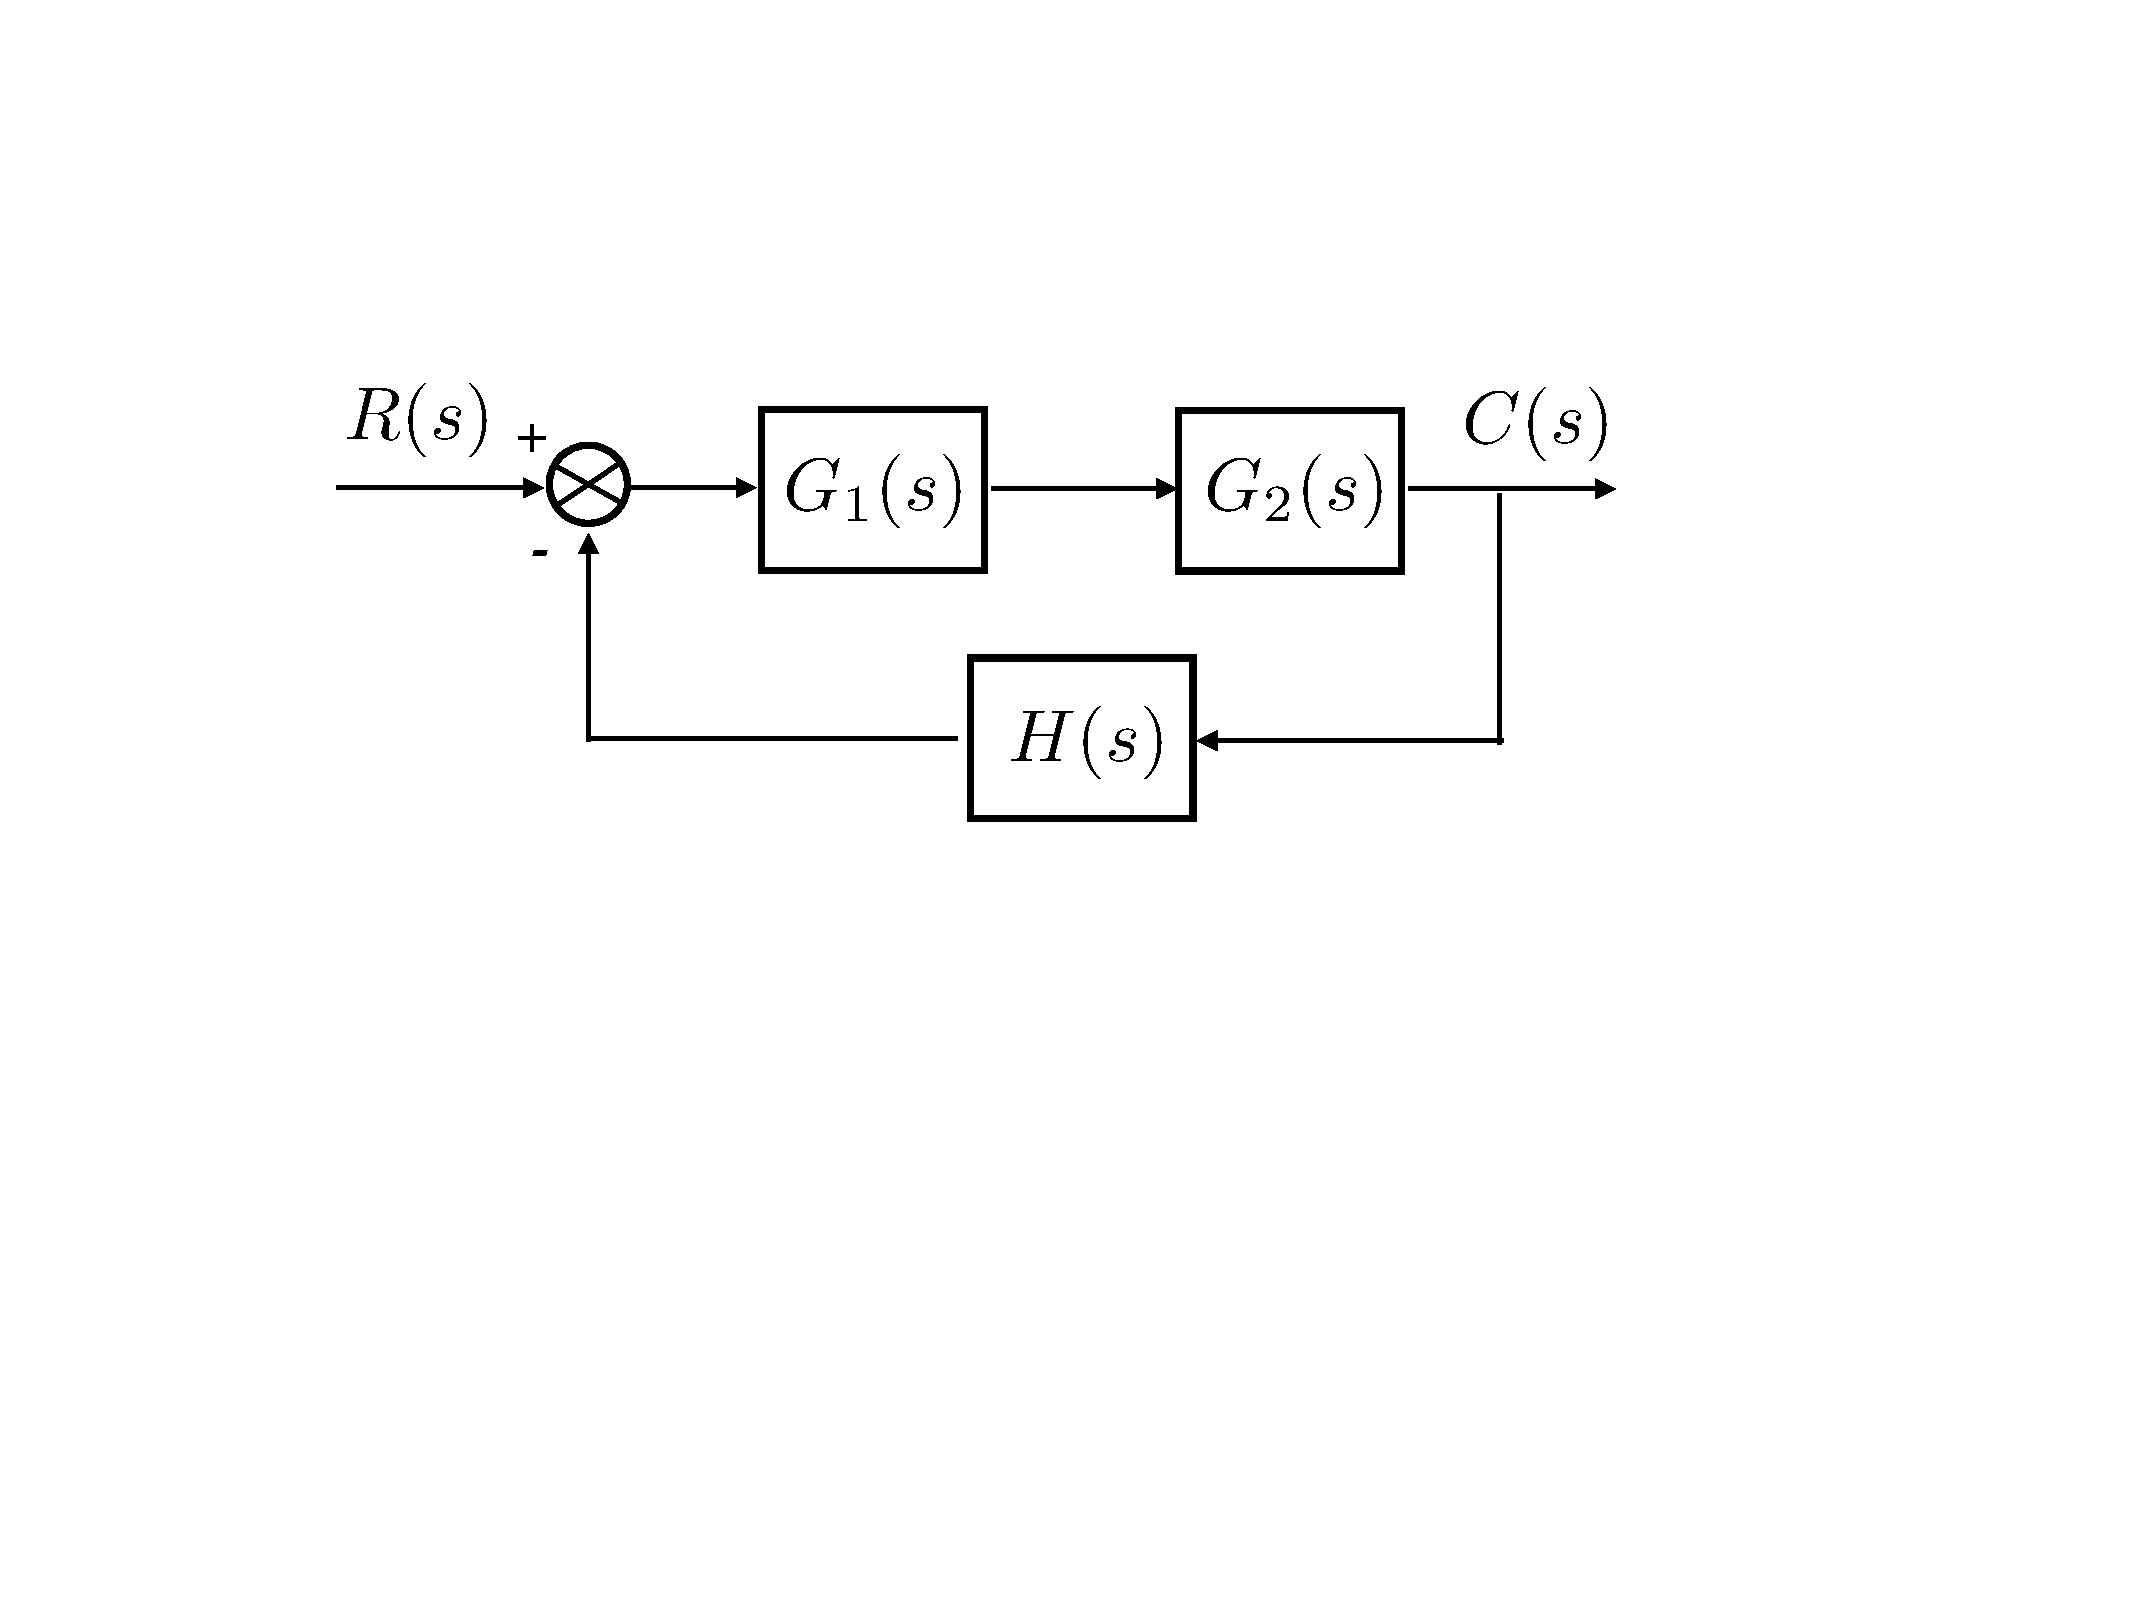
\includegraphics[width=0.55\textwidth]{Figures/FB_general} \end{center}
 \vskip-0.5cm\caption{Negative feedback system.}
\label{fig:ex}
\end{figure}

\subsection*{Solution 1}
\begin{enumerate}
	\item Primeiramente, é necessário achar os polos e os zeros. Com isso, verificando seus angulos, achamos os trechos sobre o eixo real que correspondem ao espaço das raizes. Depois, procura-se as assintotas do sistema, calculado através de seus polos e zeros. Depois, devemos achar os pontos de break away e break-in. Para tal, utilizamos a relação $\cfrac{dK}{ds}=0$, obtida através de $1+G(s)H(s)=0$.Por fim, achamos onde o \textit{Root Locus} cruza o eixo imaginário. Para tal, achamos o máximo ganho($K$) para qual o sistema se mantém marginalmente estável, usando qualquer método para tal (Tabela de Routh ou substituição de $jw$ na função de transferência). Com isso, conseguimos ter um esboço do gráfico da função.\\
	Já no MATLAB, precisamos apenas modelar a função de transferência e aplicar a função \textit{rlocus}.
	
	\begin{figure}[!h]  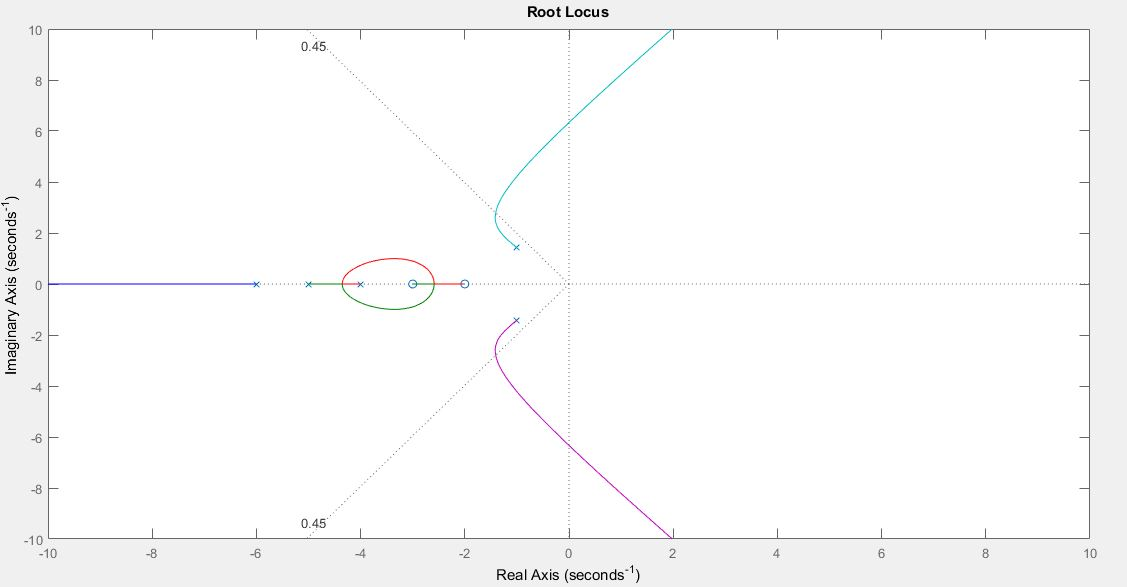
\includegraphics [scale=0.45] {Figures/exercise1-1} \end{figure}
	
	\item Usando a função \textit{rlocusfind}, achamos os pontos $-1.4056 \pm 2.7923i$ com ganho $K = 61.6824$.
	\item Usando a função \textit{rlocusfind}, achamos os pontos $\pm6.3316i$ com ganho $K = 444.0072$.
	\item $1+KG(s)H(s)=0 \longrightarrow K = \cfrac{-1}{G(s)}$
	\vskip0.4cm
	As raízes do numerador e do denominador de $\cfrac{dK}{ds}$ identificam, respectivamente, os pontos break-in e o breakaway.
	\vskip0.4cm
	\item O sistema só será estável quando estiver na parte real à esquerda do eixo imaginário, ou seja, na parte negativo do eixo real. Sendo assim, como no limiar o $K=444.0072$ (verificado no item 3), o intervalo de $K$ que o sistema será estável é $0<K<444.0072$ 
\end{enumerate}
\begin{lstlisting}
%%Exercise 1
clear all;clc;

syms s;
num = [1 5 6];
f1 = [1 6];
f2 = [1 2 3];
f3 = [1 9 20];
den = conv(f1,conv(f2,f3));
G = tf(num,den);

rlocus(G)
% axis([-1.7 -1.2 2.6 3.2])    
%Eixo para selecionar melhor o ponto zeta=0.45
% axis([-0.01 0.01 6.31 6.35]) 
%Eixo para selecionar melhor o ponto onde cruza o eixo imaginario
axis([-10 10 -10 10])
z=0.45; wn=0;
sgrid(z,wn)
[k,p] = rlocfind(G)
\end{lstlisting}
%%%%%%%%%% Ex 2 %%%%%%%%%%%
{\Large \noindent \bf Exercise 2} \hfill					25 Points\\

\noindent Consider the negative feedback system shown in Figure \ref{fig:ex}. For this system, the transfer functions, $G_1(s), G_2(s)$ and $H(s)$, are given in equation \ref{eq:ex2}.
  
\begin{equation}
G_1=10, \, G_2(s)=\cfrac{s^2+3s+2}{s^2(s^3+15s^2+74s+120)} \ \text{and} \, H(s)=\cfrac{s+6}{s^2+17s+72}
\label{eq:ex2}
\end{equation} 
  
 \noindent Do the following:
\begin{enumerate}
\item Define the system type.
\item Define the static error constants. 
\item Find the steady-state error for the inputs $10u(t)$ and $10tu(t)$.  
\end{enumerate}
\subsection*{Solution 2}
\begin{enumerate}
	\item $G(s)=\cfrac{10 s^4 + 200 s^3 + 1250 s^2 + 2500 s + 1440}{s^7 + 32 s^6 + 401 s^5 + 2448 s^4 + 7178 s^3 + 7480 s^2 - 2300 s - 1320} $
	\vskip0.4cm
	Logo, o sistema é do tipo 0.
	\item $K_p =\lim\limits_{s\to0}G(s) = -\cfrac{12}{11} = -1.0909$\\
	$ K_v = \lim\limits_{s\to0}sG(s) = 0 $\\
	$ K_a = \lim\limits_{s\to0}s^2G(s) = 0 $\\
	\item $\text{SSError}_1 = \cfrac{10}{1 + K_p} = -110 $
	\vskip0.4cm
	$\text{SSError}_2 = \cfrac{10}{K_v} = \infty$
\end{enumerate}
\begin{lstlisting}
%% Exercise2
%2.1 e 2.2
clear all;clc;

G1 = tf(10);

f1 = [1 3 2];
f2 = [1 0 0];
f3 = [1 15 74 120];
G2 = tf(f1,conv(f2,f3));

f4 = [1 6];
f5 = [1 17 72];
H = tf(f4,f5);

T = feedback(G1*G2,H);
G = T /(1-T);
G = minreal(G)
Kp = dcgain(G)

error = 10 / (1 + Kp)
\end{lstlisting}
%%%%%%%%%% Ex 3 %%%%%%%%%%%
\vskip0.3cm

{\Large \noindent \bf Exercise 3} \hfill					25 Points\\

\noindent Consider the negative feedback system shown in Figure \ref{fig:ex}. For this system, the transfer functions, $G_2(s)$ and $H(s)$, are given in equation \ref{eq:ex3}.

\begin{equation}
G_2(s)=\cfrac{1}{(s+1)(s-2)(s+3)} \ \text{and} \ H(s)=1
\label{eq:ex3}
\end{equation}
\vskip0.1cm
\noindent Using the root locus, the goal is to design a controller that stabilises the process and provides a settling time of less than 2 seconds. 
\begin{enumerate}
\item Among the following possible controllers, define which one satisfies the required conditions.
\begin{enumerate}
\item $G_1=K$;
\item $G_1=\cfrac{K(s+1)}{(s+a)}$, where $a=10$;
\item $G_1=\cfrac{K(s+1)(s+3)}{(s+a)^2}$, where $a=15$.
\end{enumerate}
\item Discuss and motivate your choices.
\end{enumerate}
\subsection*{Solution 3}
Para cada um dos itens, plotamos o \textit{Root Locus} correspondente. Assim, temos:
\begin{figure}[H]
	\makebox[\textwidth][c]{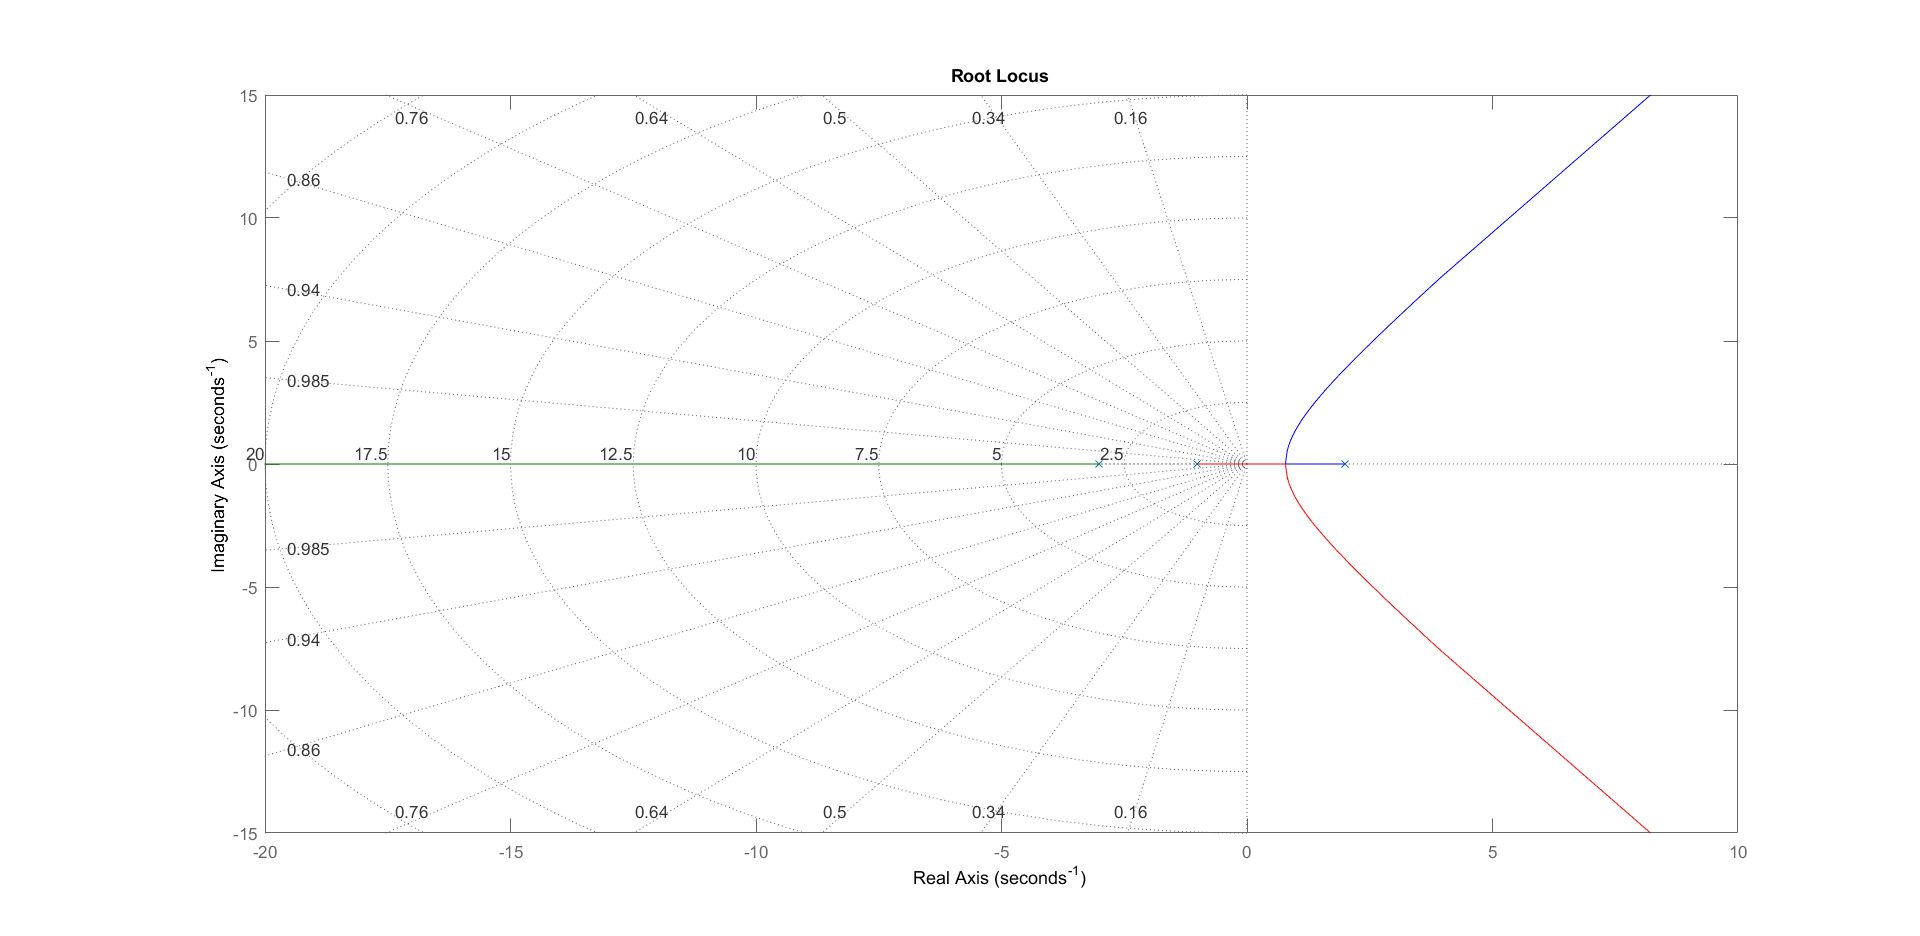
\includegraphics[scale=0.4]{Figures/exercise3-1}}
	\caption{Root Locus a}
	\label{fig:key}
\end{figure}

Nesse primeiro \textit{Root Locus}, verificamos que as raizes positivas estáveis estão todas sobre o eixo real. Desse modo, todas tem $\zeta = 1$, o que caracteriza um sistema criticamente amortecido. Tal sistema é ideal, e não existe no mundo real. Logo, é desconsiderado para nosso controlador.

\begin{figure}[H]
	\makebox[\textwidth][c]{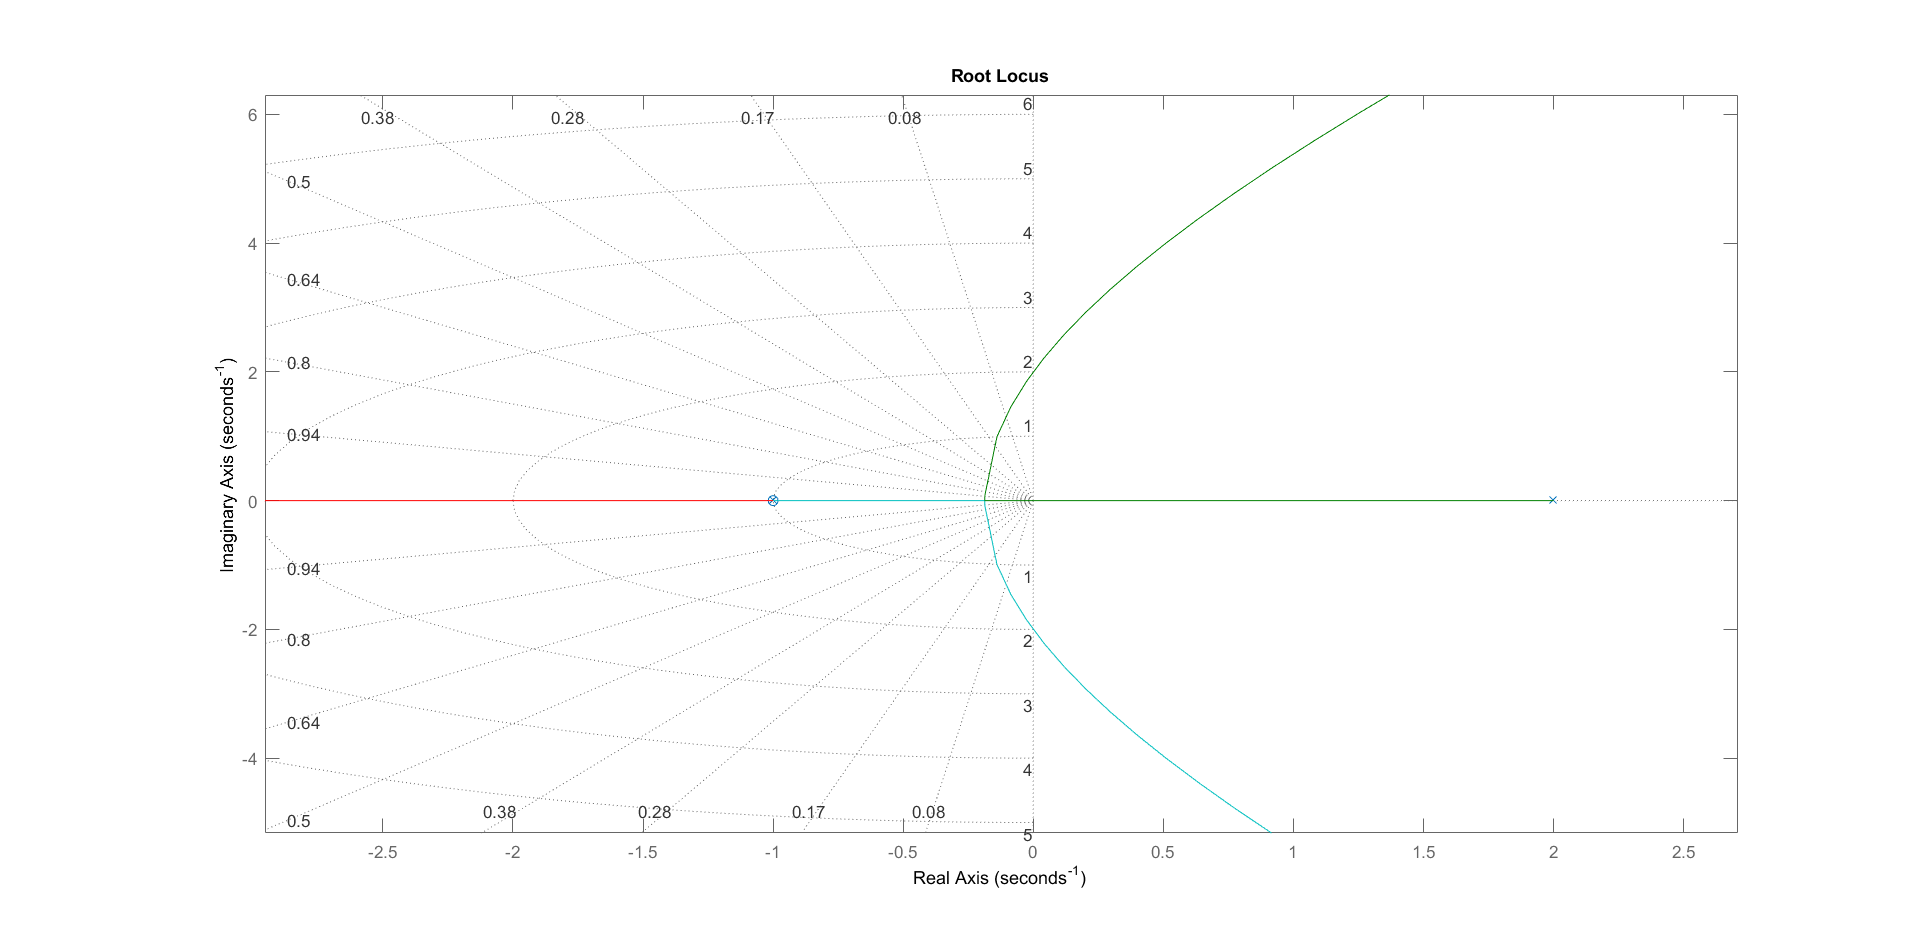
\includegraphics[scale=0.4]{Figures/exercise3-2}}
	\caption{Root Locus b}
	\label{fig:key}
\end{figure}

Já no segundo \textit{Root Locus}, temos raizes no plano esquerdo ao eixo imaginário com $\zeta \neq 1$, que caracteriza sistemas amortecidos. Sabemos que $ \zeta = \cos\theta$, com isso $0<\zeta<1$. Logo, como $T_s=\cfrac{4}{\zeta w_n} $, temos que $T_s<2\text{ segundos}$, somente se $w_n>2$. Contudo, analisando os pontos no gráfico, encontramos que o maior $w_n$ estável é menor ou igual a 2, em uma situação que o $\zeta$ é quase 0. Com isso, ainda não é o controlador ideal para nosso problema, pois seu $ T_s$ ainda é maior que 2.

\begin{figure}[H]
	\makebox[\textwidth][c]{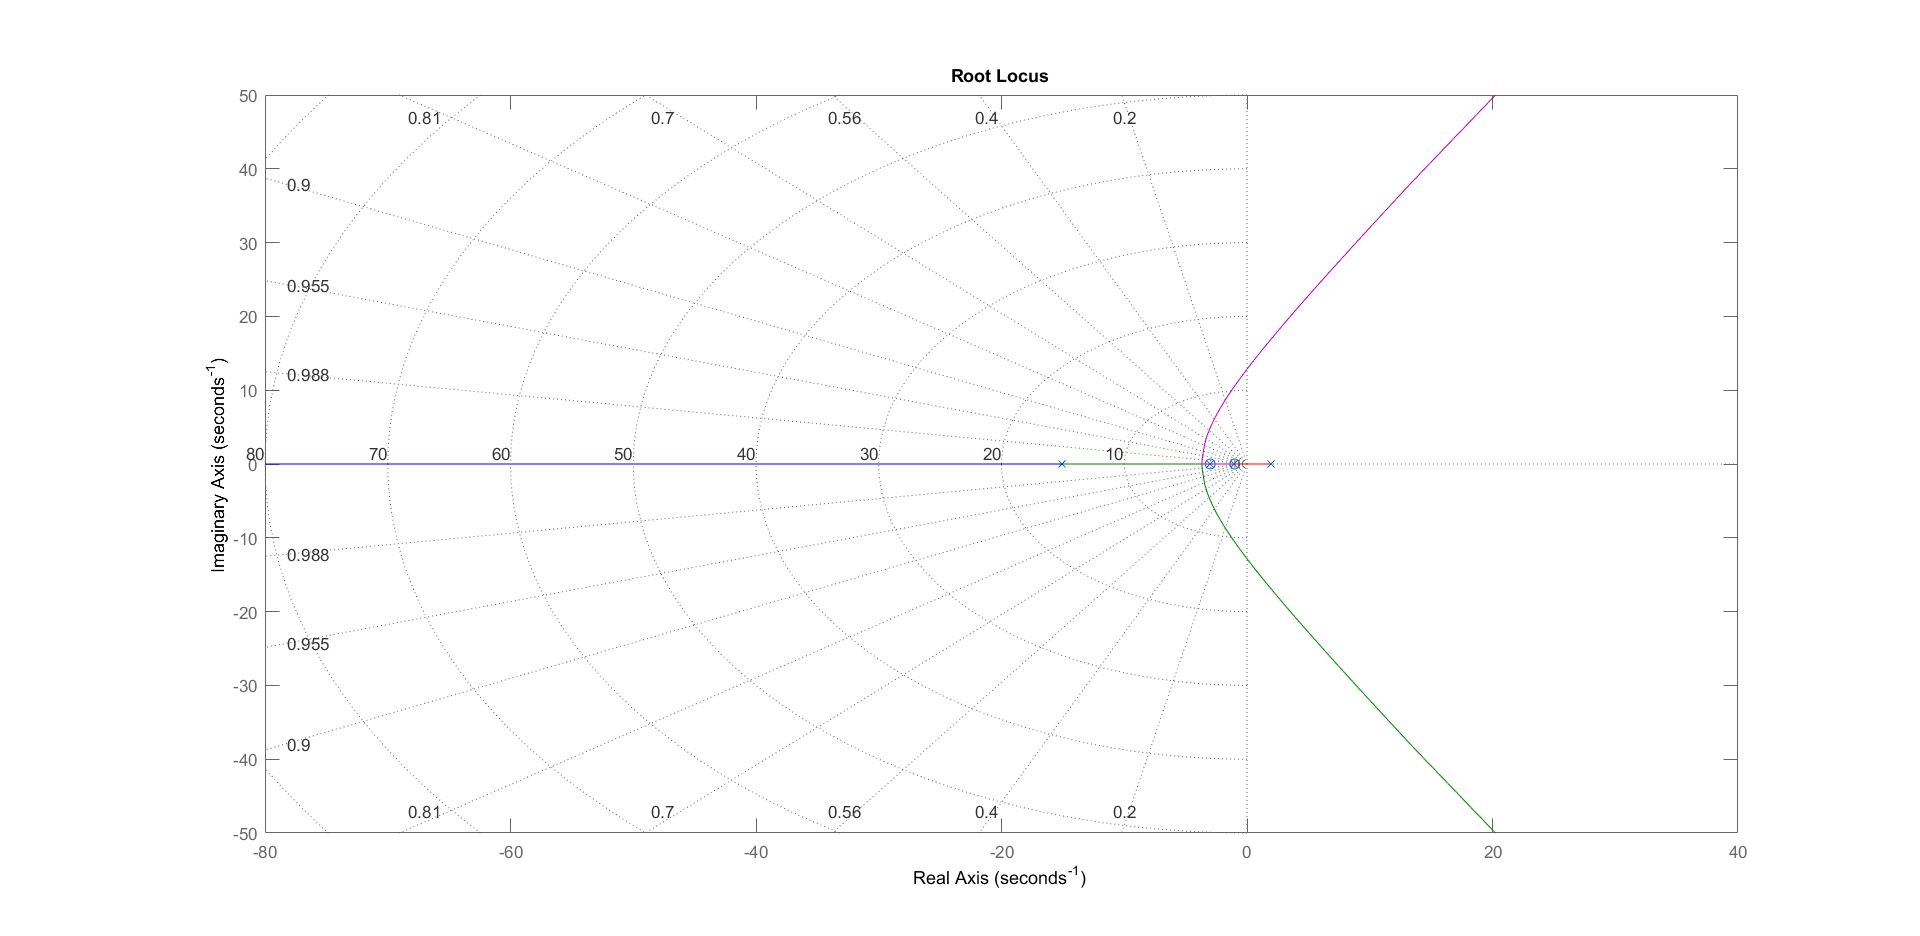
\includegraphics[scale=0.4]{Figures/exercise3-3}}
	\caption{Root Locus b}
	\label{fig:key}
\end{figure}

No último caso, também temos raizes no plano esquerdo ao eixo imaginário com $\zeta\neq1$. Contudo, percebemos que tais raizes estão mais distantes do eixo imaginário, de modo que alcançam frequências $w_n$ mais elevadas. Verificando os dados do gráfico, observamos que $3.67<w_n<12.8$. Com isso, existem vários ganhos que satisfazendo o tempo de estabilização desejado para o nosso controlador, sendo esse intervalo aproximadamente $ 728<K<1930 $.

\begin{lstlisting}
%% Exercise3
clear all;clc;

f1 = [ 1 1]
f2 = [ 1 -2]
f3 = [ 1 3]
den = conv(f1,conv(f2,f3))
G1=tf(1,den)

figure(1);
rlocus(G1)
grid on;

T2 = tf([1 1],[1 10]);
G2 = G1 * T2
figure(2);
rlocus(G2)
grid on;

T3 = tf(conv([1 1],[1 3]),[1 30 225]);
G3 = G1 * T3
figure(3);
rlocus(G3)
grid on;
\end{lstlisting}
%%%%%%%%%% Ex 4 %%%%%%%%%%%
\vskip1cm

{\Large \noindent \bf Exercise 4} \hfill					25 Points\\

\noindent Consider the negative feedback system shown in Figure \ref{fig:ex}. For this system, the transfer functions, $G_1(s), G_2(s)$ and $H(s)$, are given in equation \ref{eq:ex4}.
\begin{equation}
G_1=20, \ G_2(s)=\cfrac{1}{(1+10s)(1+2s)(1+0.2s)} \ \text{and} \ H(s)=1
\label{eq:ex4}
\end{equation} 

\noindent Do the following:
\begin{enumerate}
\item Sketch the Bode asymptotic magnitude and asymptotic phase plots.
\item Sketch the Nyquist diagram for the system.
\item Comment the plots.
\end{enumerate}
\subsection*{Solution 4}
\begin{enumerate}
	\item
	\vskip0.4cm
	\begin{figure}[H]  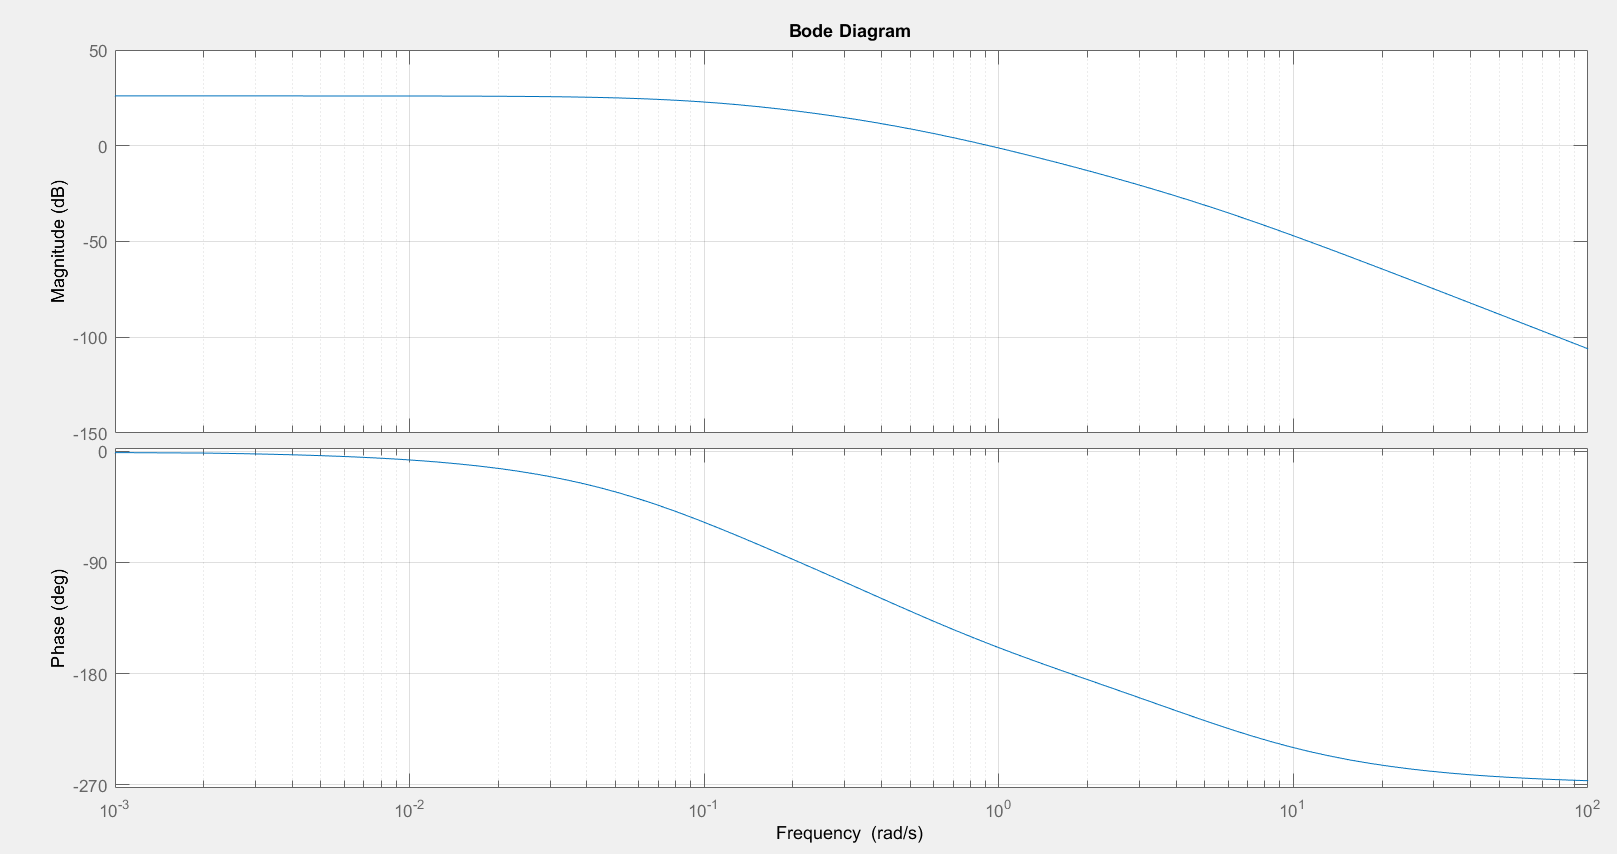
\includegraphics [scale=0.45] {Figures/exercise4-1} \end{figure}
	\item 
	\vskip0.4cm
	\begin{figure}[H]  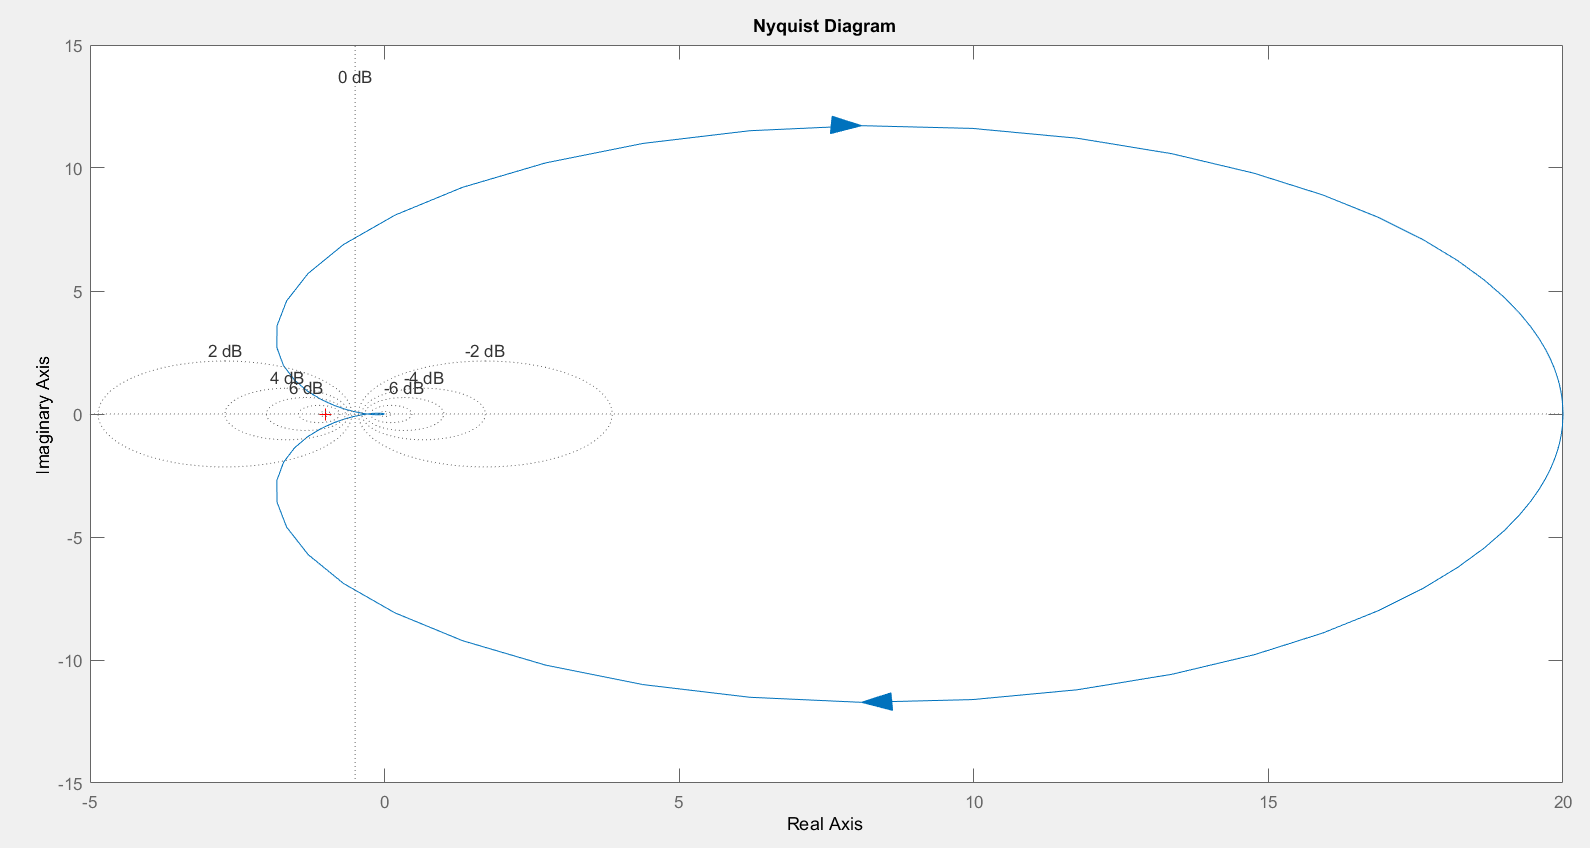
\includegraphics [scale=0.45] {Figures/exercise4-2} \end{figure}
\end{enumerate}

\begin{lstlisting}
%% Exercise4
clear all;clc;

G1 = tf(20)

f1 = [ 10 1 ]
f2 = [ 2 1 ]
f3 = [ 0.2 1 ]

G2 = tf(1,conv(f1,conv(f2,f3)))

G = G1*G2

figure(1);
bode(G)
grid on;

figure(2);
nyquist(G)
grid on;
\end{lstlisting}
%%%%%%%%%% Ex 5 %%%%%%%%%%%
\vskip0.8cm
{\Large \noindent \bf Exercise 5} \hfill					20 Points ({\sc Extra}) \\

\noindent  Consider the two-tank system given in HW1.\\
 
\begin{figure}[ht!]
\begin{center}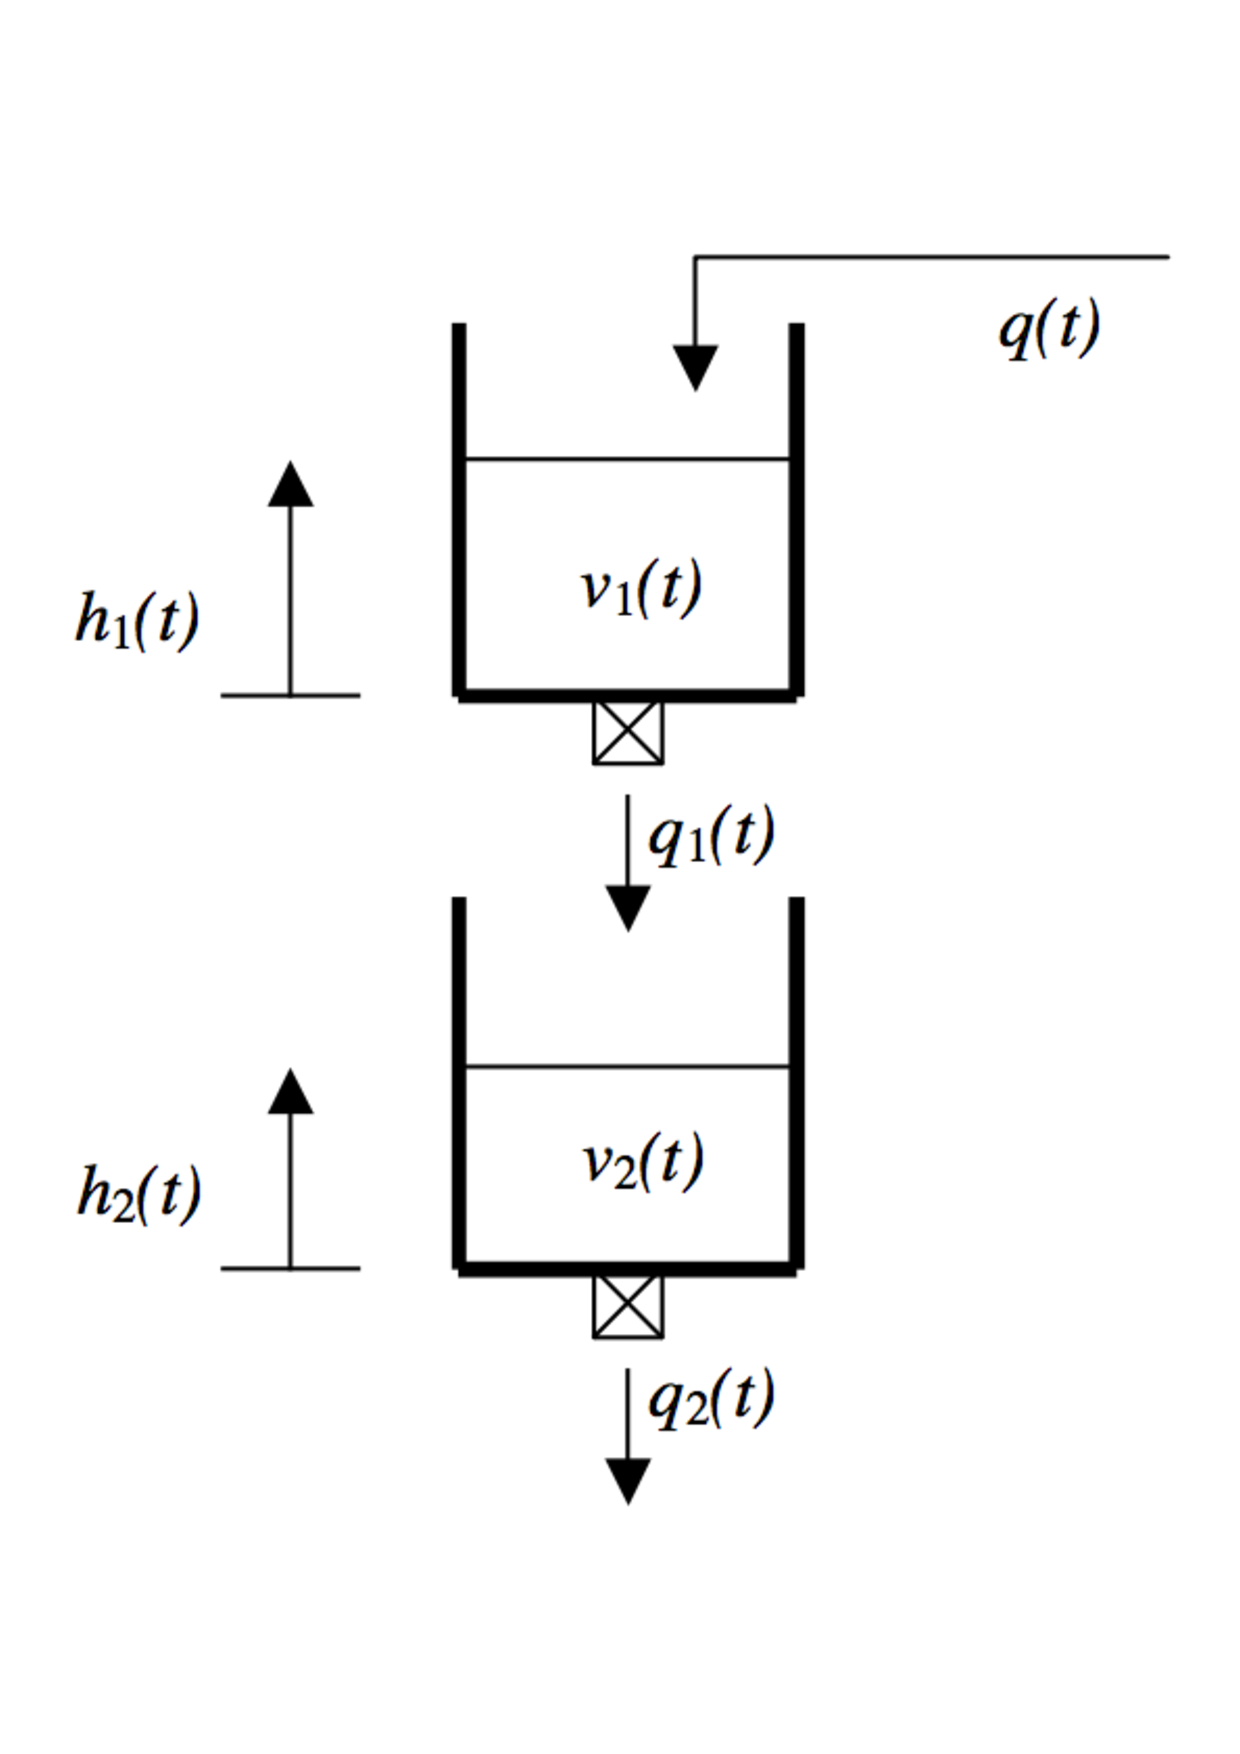
\includegraphics[width=0.44\textwidth]{Figures/tanks_ex} \end{center}
 \vskip-0.5cm\caption{Two-tank system for Exercise 5.}
\label{fig:ex3}
\end{figure}

\noindent  The liquid inflow to the first tank, $u(t)=q_0(t)$, can be controlled using a valve. The upper tank's outflow, $q_1(t)$, equals the lower tank's inflow. The outflow of the lower tank is  $q_2(t)$. The objective of the design is to control the liquid level, $y(t)=h_2(t)$, in the lower tank. 

\begin{enumerate}
\item Given the cross-sectional areas $S_1=2$ and $S_2=4$ [m$^2$] and the coefficients $K_1=3$,  $K_2=4$  for the upper and lower tanks, verify that the open loop transfer function for this system can be written as:
\begin{equation*}
\cfrac{Y(s)}{Q_0(s)}=\cfrac{a_1/a_3}{s^2+(a_1+a_2)s+a_1a_2}
\end{equation*}
\begin{itemize}
\item where $a_1=K_1/S_1, \  a_2=K_2/S_2$ and $a_3=S_2$.
\end{itemize}
\item The system is operating at 10\% overshoot. Design a controller to reduce by half the system's settling time.
\item Discuss and justify your choices.
\item Verify your design through Matlab/Octave simulations.
\end{enumerate}
\subsection*{Solution 5}
\begin{enumerate}
	\item 
	\item PD$= s + 6.5538 $
	\item Usando o MATLAB, calculamos os novos polos dominantes de acordo com o Overshoot(e consequentemente o $\zeta$) dado na questão. Com eles, podemos projetar o sistema dado acima.
	\item 
	\begin{lstlisting}
	%% Exercise 5
	clear all;clc;
	
	S1 = 2 ; S2 = 4; K1 = 3; K2 = 4;
	a1 = K1/S1 ; a2 = K2/S2 ; a3 = S2;
	numg = [ a1/a3 ]; deng = [ 1 a1+a2 a1*a2];
	G = tf( numg, deng)
	
	overshoot = 10;
	z=-log(overshoot/100)/sqrt(pi^2+[log(overshoot/100)]^2);
	% Plot uncompensated root locus
	figure(1);
	rlocus(G)
	axis([-10 10 -10 10])
	% Overlay desired percent OS line
	sgrid(z,0)
	title(['Uncompensated Root Locus with ', num2str(overshoot),'% OS Line'])
	
	%Generate gain, K, and closed-loop poles, p, for point selected ...
	%interactively on the root locus
	[K,p]=rlocfind(G)
	
	Tss0 = 4/abs(real(p(1)));
	
	% Simulate uncompensated closed-loop
	T=feedback(K*G,1) % Find uncompensated T(s)
	[y,t]=step(T); % Step response of uncompensated system
	
	Tssf = Tss0/2;
	% Calculate natural frequency
	wn=4/(Tssf*z);
	% Calculate desired dominant pole location
	desired_pole=(-z*wn)+(wn*sqrt(1-z^2)*i);
	% Calculate angular contribution to desired pole without PD compensator
	angle_at_desired_pole=(180/pi)*...
	angle(polyval(numg,desired_pole)/polyval(deng,desired_pole));
	% Calculate required angular contribution from PD compensator
	PD_angle=180-angle_at_desired_pole;
	% Calculate PD zero location
	zc=((imag(desired_pole)/tan(PD_angle*pi/180))-real(desired_pole));
	
	% PD Compensator
	numc=[1 zc]; % Calculate numerator of Gc(s)
	denc=[0 1]; % Calculate denominator of Gc(s)
	Gc=tf(numc,denc) % Create and display Gc(s)
	Ge=G*Gc % Cascade G(s) and Gc(s)
	
	% Plot compensated root locus
	figure(2);
	rlocus(Ge)
	axis([-10 10 -10 10])
	sgrid(z,0) % Overlay desired % OS line
	title(['PD Compensated Root Locus with ' , num2str(overshoot),'% OS Line'])
	
	[K,p]=rlocfind(Ge)
	Tssprat =4/abs(real(p(1)))
	
	% PD compensated system
	Tc=feedback(K*Ge,1) % PD compensated T(s).
	[yc,tc]=step(Tc,t); % Step response for PD compensated system.
	
	% Compare
	figure(3);
	plot(tc,yc,'LineWidth', 1.5); hold on; axis tight
	plot(t,y, 'LineWidth', 1.5, 'Color','r'); grid on
	legend('Compensated', 'Uncompensated')
	title('System response comparison')
	set(gca,'FontSize',12)
	hold off
	\end{lstlisting}
	\begin{figure}[H]  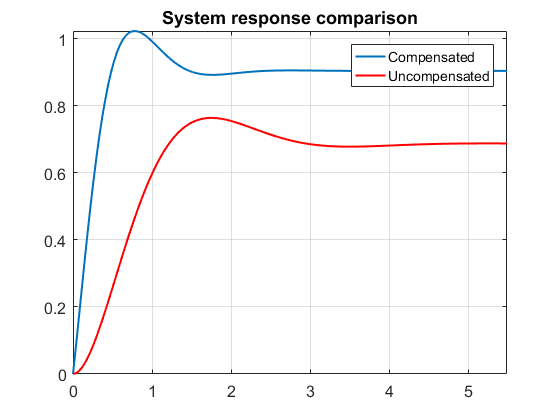
\includegraphics [scale=0.9] {Figures/exercise5} \end{figure}
\end{enumerate}
\end{document}